
%%%%%%%%%%%%%%%%%%%%%%% file typeinst.tex %%%%%%%%%%%%%%%%%%%%%%%%%
%
% This is the LaTeX source for the TDPTemplate using
% the LaTeX document class 'llncs.cls' Springer LNAI format
% used in the RoboCup Symposium submissions.
% http://www.springer.com/computer/lncs?SGWID=0-164-6-793341-0
%
% It may be used as a template for your own TDP - copy it
% to a new file with a new name and use it as the basis
% for your Team Description Paper
%
% NB: the document class 'llncs' has its own and detailed documentation, see
% ftp://ftp.springer.de/data/pubftp/pub/tex/latex/llncs/latex2e/llncsdoc.pdf
%
%%%%%%%%%%%%%%%%%%%%%%%%%%%%%%%%%%%%%%%%%%%%%%%%%%%%%%%%%%%%%%%%%%%

\documentclass[runningheads,a4paper]{llncs}
\usepackage{amssymb}
\setcounter{tocdepth}{3}
\usepackage{graphicx}
\usepackage{amssymb}
\usepackage[utf8]{inputenc}
\usepackage{url}
\usepackage{float}
\usepackage{amsmath}
\usepackage{graphicx}
\usepackage{wrapfig}
\usepackage{fancyhdr}

\pagestyle{empty}
\pagestyle{fancy}
\begin{document}

\title{Team-Name 2015 Team Description Paper}

\author{Team Leader \and Team Member-1 \and Team Member-2 \and Team Member-3 \and So on...}
\institute{[Intitute name and direction here], \\
\texttt{http://devoted-web-site.url}}
\maketitle


%%%%%%%%%%%%%%%%%%%%%%%%%%%%%%%%%%%%%%%%%%%%%%%%%%%%%%%%%%%%%%%%%%%%%%%%%%%%%%%%%%%%

\begin{abstract}

In your abstract, please state which is the main research line of your team for this year (on which problem or set of problems are you focusing all the team efforts). Tell why this research is important, how are you approaching to the problem solution and which results do you expect to obtain.

\end{abstract}


%%%%%%%%%%%%%%%%%%%%%%%%%%%%%%%%%%%%%%%%%%%%%%%%%%%%%%%%%%%%%%%%%%%%%%%%%%%%%%%%%%%%

\section{Robot's Hardware Brief Description}
Please describe in this section your robot's configuration and hardware. Consider the following example:

\begin{wrapfigure}[13]{r}{0.45\textwidth}
	\vspace*{-1cm}
	\centering
	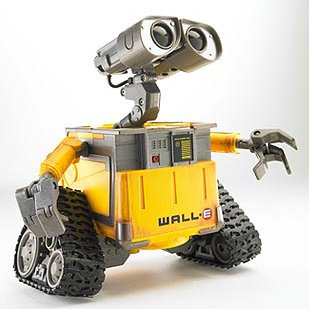
\includegraphics[width=0.4\textwidth]{images/robot.jpg}
	\caption{Robot picture}
	\label{fig:virbot}
\end{wrapfigure}
\textit{The robot has an anthropomorphic design built over a Pioneer PatrolBot base. Specifications are as follows:}
\begin{itemize}
	\item Base: Pioneer PatrolBot (differential pair), 0.5m/s max speed.
	\item Torso: Home-made. 1 DOF (elevation) prismatic to change the robot height between 1.0 to 1.7m.
	\item Left arm: Mounted on torso. 7 DOF, anthropomorphic, home-made. Maximum load: 1kg.
	\item Right arm: Mounted on torso. 7 DOF, anthropomorphic, home-made. Maximum load: 1kg.
	\item Head: 2DOF (pan \& tilt), home-made.
	\item External devices: None
	\item Robot dimensions: height: 1.7m (max), width: 0.7m depth 0.8m
	\item Robot weight: 50kg.
\end{itemize}

\textit{Also our robot incorporates the following devices:}

\begin{itemize}
	\item Array of sonars mounted on base
	\item Hokuyo UHG 04LX(Laser Range Finder) on base and chest
	\item Kinect device mounted on head
	\item 10Mpx camera mounted on head
	\item Directional microphone
	\item On-board speakers
	\item Pressure sensors on each hand (arms)
	\item 2 Intel i5 laptops
\end{itemize}

\section{Robot's Software Description}
Please describe in this section the software you are using to control your robot.
Consider the following example:

\textit{For our robot we are using the following software:}

\begin{itemize}
	\item Platform: ROS
	\item Navigation, localization and mapping: ROS
	\item Face recognition: Home-made. Please refer to [1, 2, 3]
	\item Speech recognition: Sphinx
	\item Speech generation: Festival
	\item Object recognition: Home-made. Please refer to [4, 5, 6]
	\item Arms control and two-hand coordination: Home-made, see description on following sections.
\end{itemize}

\section*{Team research}
In the following sections you are free to describe your work. Please focus on your current research and state clear its scientific contribution value and why it is important for you and the league. The length of the TDP is limited to 8 pages.

Remember that the TDP must contain the following information:

\begin{itemize}
	\item Description of the hardware and software including a list of integrated externally available components (including commercial products, freeware, Open Source, etc.)
	\item Innovative technology and scientific contribution
	\item Photo(s) of the robot
	\item Focus of research/research interests
	\item Re-usability of the system for other research groups
	\item Applicability of the robot in the real world
\end{itemize}

\section*{Bibliography}
Add your references here
%\bibliographystyle{unsrt}
%\bibliography{bibliography}
\end{document} 